\documentclass{scrartcl}\usepackage{graphicx, color}
%% maxwidth is the original width if it is less than linewidth
%% otherwise use linewidth (to make sure the graphics do not exceed the margin)
\makeatletter
\def\maxwidth{ %
  \ifdim\Gin@nat@width>\linewidth
    \linewidth
  \else
    \Gin@nat@width
  \fi
}
\makeatother

\definecolor{fgcolor}{rgb}{0.2, 0.2, 0.2}
\newcommand{\hlnumber}[1]{\textcolor[rgb]{0,0,0}{#1}}%
\newcommand{\hlfunctioncall}[1]{\textcolor[rgb]{0.501960784313725,0,0.329411764705882}{\textbf{#1}}}%
\newcommand{\hlstring}[1]{\textcolor[rgb]{0.6,0.6,1}{#1}}%
\newcommand{\hlkeyword}[1]{\textcolor[rgb]{0,0,0}{\textbf{#1}}}%
\newcommand{\hlargument}[1]{\textcolor[rgb]{0.690196078431373,0.250980392156863,0.0196078431372549}{#1}}%
\newcommand{\hlcomment}[1]{\textcolor[rgb]{0.180392156862745,0.6,0.341176470588235}{#1}}%
\newcommand{\hlroxygencomment}[1]{\textcolor[rgb]{0.43921568627451,0.47843137254902,0.701960784313725}{#1}}%
\newcommand{\hlformalargs}[1]{\textcolor[rgb]{0.690196078431373,0.250980392156863,0.0196078431372549}{#1}}%
\newcommand{\hleqformalargs}[1]{\textcolor[rgb]{0.690196078431373,0.250980392156863,0.0196078431372549}{#1}}%
\newcommand{\hlassignement}[1]{\textcolor[rgb]{0,0,0}{\textbf{#1}}}%
\newcommand{\hlpackage}[1]{\textcolor[rgb]{0.588235294117647,0.709803921568627,0.145098039215686}{#1}}%
\newcommand{\hlslot}[1]{\textit{#1}}%
\newcommand{\hlsymbol}[1]{\textcolor[rgb]{0,0,0}{#1}}%
\newcommand{\hlprompt}[1]{\textcolor[rgb]{0.2,0.2,0.2}{#1}}%

\usepackage{framed}
\makeatletter
\newenvironment{kframe}{%
 \def\at@end@of@kframe{}%
 \ifinner\ifhmode%
  \def\at@end@of@kframe{\end{minipage}}%
  \begin{minipage}{\columnwidth}%
 \fi\fi%
 \def\FrameCommand##1{\hskip\@totalleftmargin \hskip-\fboxsep
 \colorbox{shadecolor}{##1}\hskip-\fboxsep
     % There is no \\@totalrightmargin, so:
     \hskip-\linewidth \hskip-\@totalleftmargin \hskip\columnwidth}%
 \MakeFramed {\advance\hsize-\width
   \@totalleftmargin\z@ \linewidth\hsize
   \@setminipage}}%
 {\par\unskip\endMakeFramed%
 \at@end@of@kframe}
\makeatother

\definecolor{shadecolor}{rgb}{.97, .97, .97}
\definecolor{messagecolor}{rgb}{0, 0, 0}
\definecolor{warningcolor}{rgb}{1, 0, 1}
\definecolor{errorcolor}{rgb}{1, 0, 0}
\newenvironment{knitrout}{}{} % an empty environment to be redefined in TeX

\usepackage{alltt} % A wider text than  \documentclass{article} 


% Configure hyper links
\usepackage{hyperref} 
\hypersetup{
  colorlinks   = true, %Colours links instead of ugly boxes
  urlcolor     = blue, %Colour for external hyperlinks
  linkcolor    = black, %Colour of internal links
  citecolor   = black %Colour of citations
}


\title{Reproducing estimates by Chas-Amil and Buongiorno in "The demand for paper and paperboard - Econometric model for the European Union"}
\author{Paul Rougieux}
\IfFileExists{upquote.sty}{\usepackage{upquote}}{}
\begin{document}
\maketitle

\begin{abstract}
Chas Amil and buongiorno (2000) estimated demand functions for paper and paperboard products in the European Union (EU15). In a first section, we attempt to reproduce their graphs and estimates for the period 1996-1992, based on FAOSTAT forest products production and trade data and World Bank GDP and deflator data. In a second section we extend the estimation period by 20 years, until 2012. In a third section, we estimate for all EU27 countries but only over the period from 1992 until 2012. 
\end{abstract}

\setcounter{tocdepth}{2}
\tableofcontents 






\newpage
\section{Reproducing Chas Amil and Buongiorno estimates for the period 1969-1995}
\subsection{Chart of Paper and Paperboard consumption}
\begin{figure}[h]
\centering
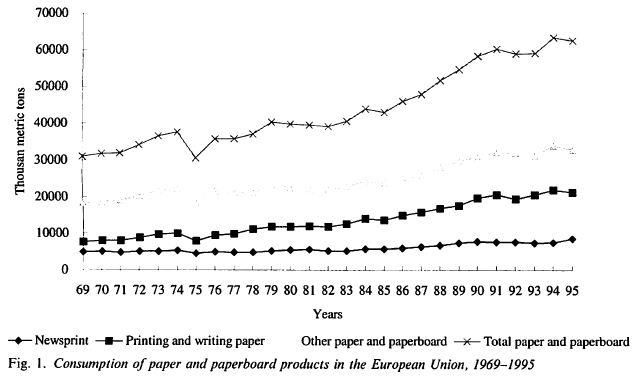
\includegraphics[width=0.7\linewidth]{./figure/ChasAmilConsumption}
\caption{Original chart reproduced from Chas Amil and Buongiorno. Consumption of paper and paperboard products in the European Union (EU15).}
\label{fig:ChasAmilConsumption}
\end{figure}

\begin{knitrout}
\definecolor{shadecolor}{rgb}{0.969, 0.969, 0.969}\color{fgcolor}\begin{figure}[h]


{\centering 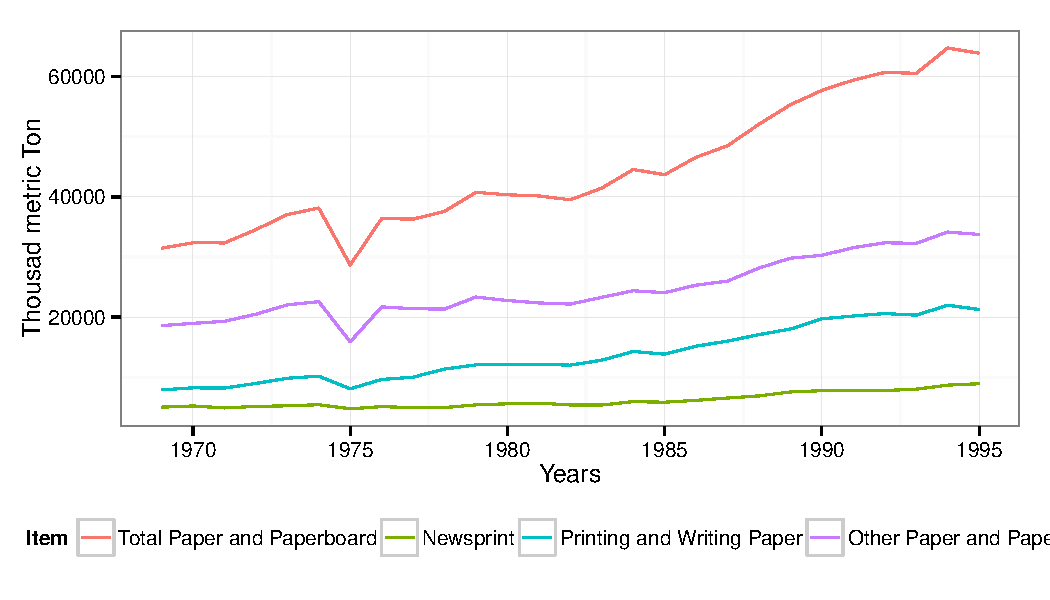
\includegraphics[width=.8\linewidth]{figure/ConsumptionEU15} 

}

\caption[Consumption of paper and paperboard products in EU15, source]{Consumption of paper and paperboard products in EU15, source: FAOSTAT\label{fig:ConsumptionEU15}}
\end{figure}


\end{knitrout}



\newpage
\subsection{Chart of paper and paperboard prices}
\begin{figure}[h]
\centering
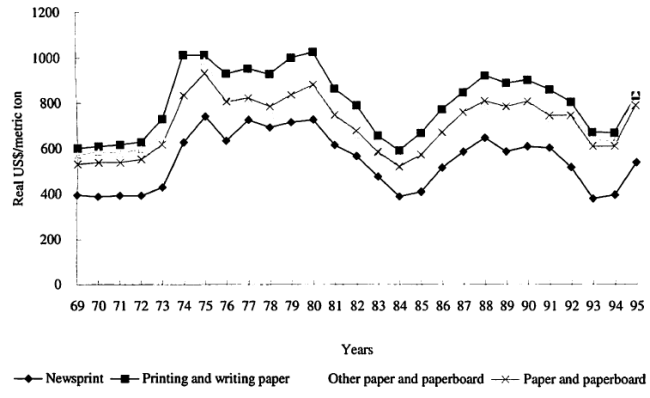
\includegraphics[width=0.6\linewidth]{./figure/ChasAmilPriceEvolution}
\caption{Original chart reproduced from Chas Amil and Buongiorno. Price Evolution of paper and paperboard products in the European Union.}
\label{fig:ChasAmilPriceEvolution}
\end{figure}

\begin{knitrout}
\definecolor{shadecolor}{rgb}{0.969, 0.969, 0.969}\color{fgcolor}\begin{figure}[h]


{\centering 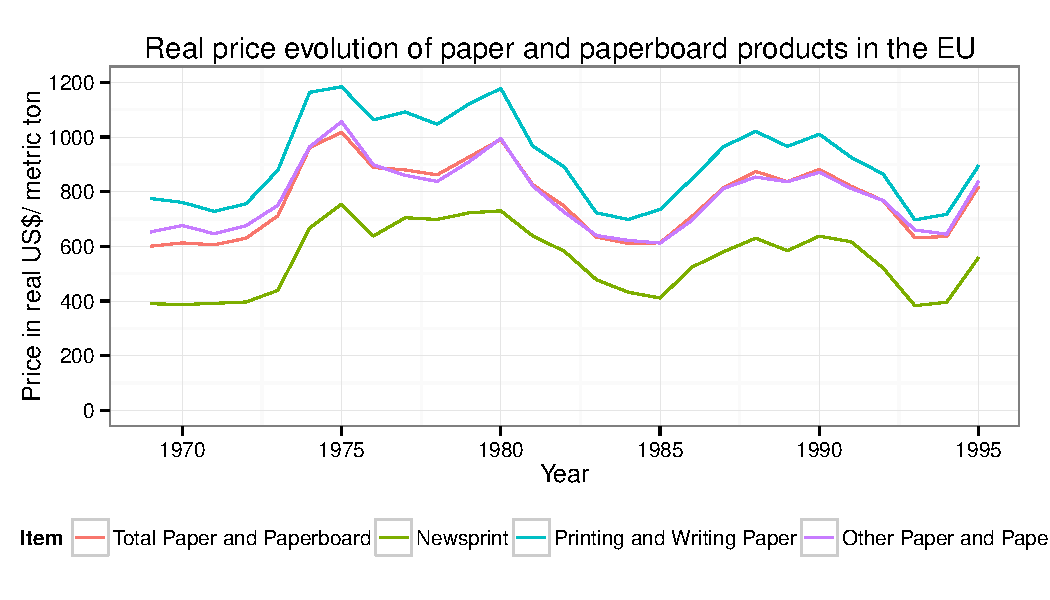
\includegraphics[width=.8\linewidth]{figure/PriceEU15} 

}

\caption[Price evolution of paper and paperboard products in EU15 in USD of 1987, source]{Price evolution of paper and paperboard products in EU15 in USD of 1987, source: FAOSTAT and own calculations.\label{fig:PriceEU15}}
\end{figure}


\end{knitrout}




\newpage
\subsection{Charts of GDP and consumption per capita}

\begin{knitrout}
\definecolor{shadecolor}{rgb}{0.969, 0.969, 0.969}\color{fgcolor}\begin{figure}[h]


{\centering 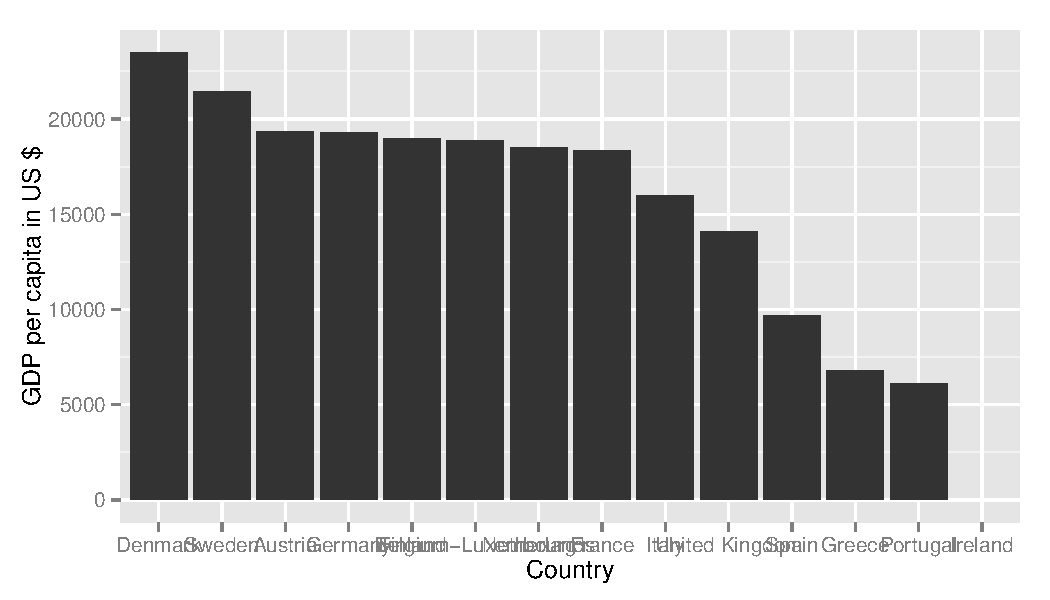
\includegraphics[width=.7\linewidth]{figure/GDPPerCapita} 

}

\caption[GDP per capita]{GDP per capita. source: World Bank.\label{fig:GDPPerCapita}}
\end{figure}


\end{knitrout}



\begin{knitrout}
\definecolor{shadecolor}{rgb}{0.969, 0.969, 0.969}\color{fgcolor}\begin{figure}[h]


{\centering 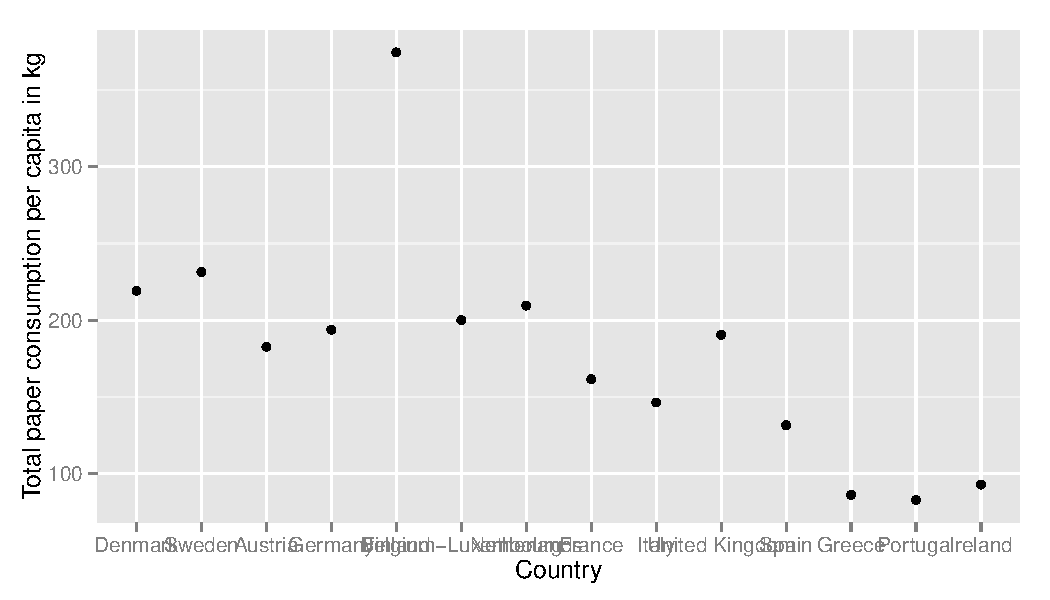
\includegraphics[width=.7\linewidth]{figure/ConsPerCapita} 

}

\caption[Paper and paperboard Consumption per capita]{Paper and paperboard Consumption per capita. source: FAOSTAT and own calculations.\label{fig:ConsPerCapita}}
\end{figure}


\end{knitrout}


\newpage
\subsection{Estimating demand functions by country}
Because the Worldbank databank doesn't contain a deflator for Ireland over the time period of interest, we couldn't calculate the GDP in constant USD for Ireland.
\begin{table}[h]
\centering
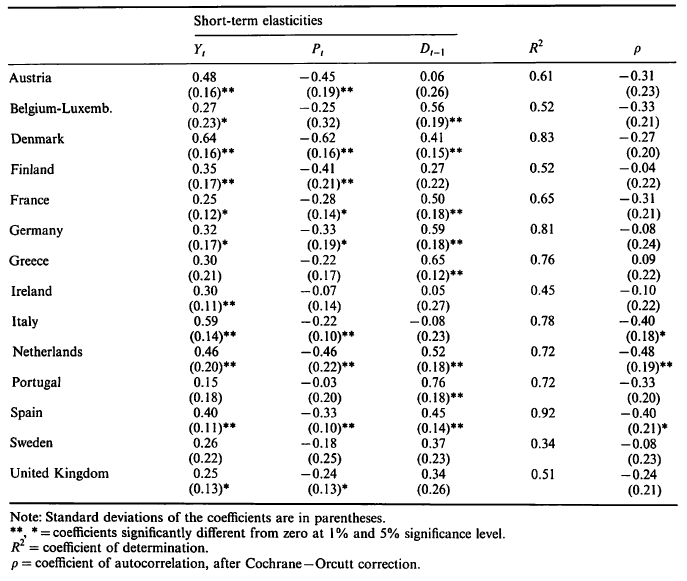
\includegraphics[width=0.7\linewidth]{./figure/ChasAmilEstimationTable1}
\caption{Original table reproduced from Chas Amil and Buongiorno. Estimates of demand equations for total paper and paperboard by country.}
\label{fig:ChasAmilEstimationTable1}
\end{table}
    

% latex table generated in R 2.15.2 by xtable 1.7-1 package
% Tue Sep 17 09:36:14 2013
\begin{table}[ht]
\centering
\begin{tabular}{rllllr}
  \hline
 & Country & Y & P & Dt\_1 & R2 \\ 
  \hline
1 & Austria & 1.52 & -0.05 & -0.22 & 0.90 \\ 
  2 &  & (0.3) & (0.09) & (0.22) &  \\ 
  3 & Belgium-Luxembourg & 1.1 & -0.09 & 0.15 & 0.88 \\ 
  4 &  & (0.3) & (0.12) & (0.22) &  \\ 
  5 & Denmark & 0.52 & -0.12 & 0.63 & 0.83 \\ 
  6 &  & (0.24) & (0.11) & (0.16) &  \\ 
  7 & Finland & 0.99 & -0.15 & 0.14 & 0.93 \\ 
  8 &  & (0.25) & (0.08) & (0.2) &  \\ 
  9 & France & 1.1 & -0.49 & -0.09 & 0.57 \\ 
  10 &  & (0.3) & (0.29) & (0.21) &  \\ 
  11 & Germany & 0.93 & -0.11 & 0.33 & 0.96 \\ 
  12 &  & (0.24) & (0.06) & (0.18) &  \\ 
  13 & Greece & 0.64 & -0.02 & 0.66 & 0.91 \\ 
  14 &  & (0.31) & (0.13) & (0.15) &  \\ 
  15 & Italy & 0.96 & 0 & 0.1 & 0.91 \\ 
  16 &  & (0.24) & (0.07) & (0.22) &  \\ 
  17 & Netherlands & 0.9 & -0.16 & 0.26 & 0.92 \\ 
  18 &  & (0.26) & (0.08) & (0.21) &  \\ 
  19 & Portugal & 0.69 & -0.12 & 0.56 & 0.91 \\ 
  20 &  & (0.32) & (0.17) & (0.21) &  \\ 
  21 & Spain & 1.66 & -0.09 & 0.07 & 0.98 \\ 
  22 &  & (0.41) & (0.05) & (0.22) &  \\ 
  23 & Sweden & 1.17 & -0.08 & -0.17 & 0.77 \\ 
  24 &  & (0.26) & (0.1) & (0.22) &  \\ 
  25 & United Kingdom & 0.51 & -0.16 & 0.45 & 0.80 \\ 
  26 &  & (0.14) & (0.07) & (0.18) &  \\ 
   \hline
\end{tabular}
\caption{Demand equations for total paper and paperboard by country} 
\label{DemandByCountry}
\end{table}


\newpage
Note: Standard deviation of the coefficients are in parentheses.
R2: Coefficient of determination.


\newpage
\subsection{Estimating demand equations for pooled countries}
\begin{table}[h]
\centering
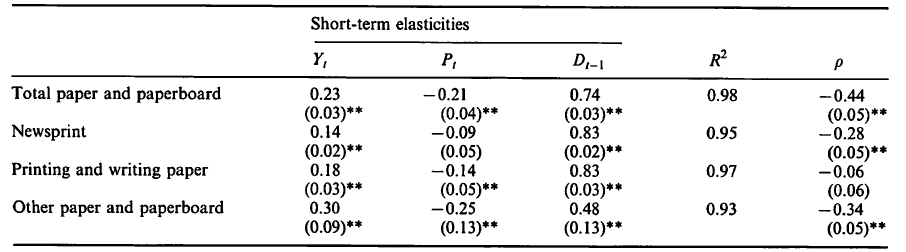
\includegraphics[width=0.7\linewidth]{./figure/ChasAmilEstimationTable2}
\caption{Original table reproduced from Chas Amil and Buongiorno. Demand equations obtained by OLS pooling for all observations 1969-1992.}
\label{fig:ChasAmilEstimationTable2}
\end{table}
    
% latex table generated in R 2.15.2 by xtable 1.7-1 package
% Tue Sep 17 09:36:14 2013
\begin{table}[ht]
\centering
\begin{tabular}{rllllr}
  \hline
 & Product & Y & P & Dt\_1 & R2 \\ 
  \hline
1 & Total Paper and Paperboard & 0.16 & -0.1 & 0.83 & 0.99 \\ 
  2 &  & (0.03) & (0.03) & (0.03) &  \\ 
  3 & Newsprint & 0.19 & -0.03 & 0.79 & 0.94 \\ 
  4 &  & (0.03) & (0.06) & (0.03) &  \\ 
  5 & Printing and Writing Paper & 0.11 & -0.05 & 0.9 & 0.98 \\ 
  6 &  & (0.03) & (0.05) & (0.03) &  \\ 
  7 & Other Paper and Paperboard & 0.34 & -0.12 & 0.63 & 0.96 \\ 
  8 &  & (0.04) & (0.05) & (0.04) &  \\ 
   \hline
\end{tabular}
\caption{Demand equations obtained by OLS pooling for all observations 1969-1992} 
\label{DemandPooled}
\end{table}





\newpage
\section{Extenting time series until 2012}
\subsection{Chart of Paper and Paperboard Consumption (1969-2012)}
\begin{knitrout}
\definecolor{shadecolor}{rgb}{0.969, 0.969, 0.969}\color{fgcolor}\begin{figure}[h]


{\centering 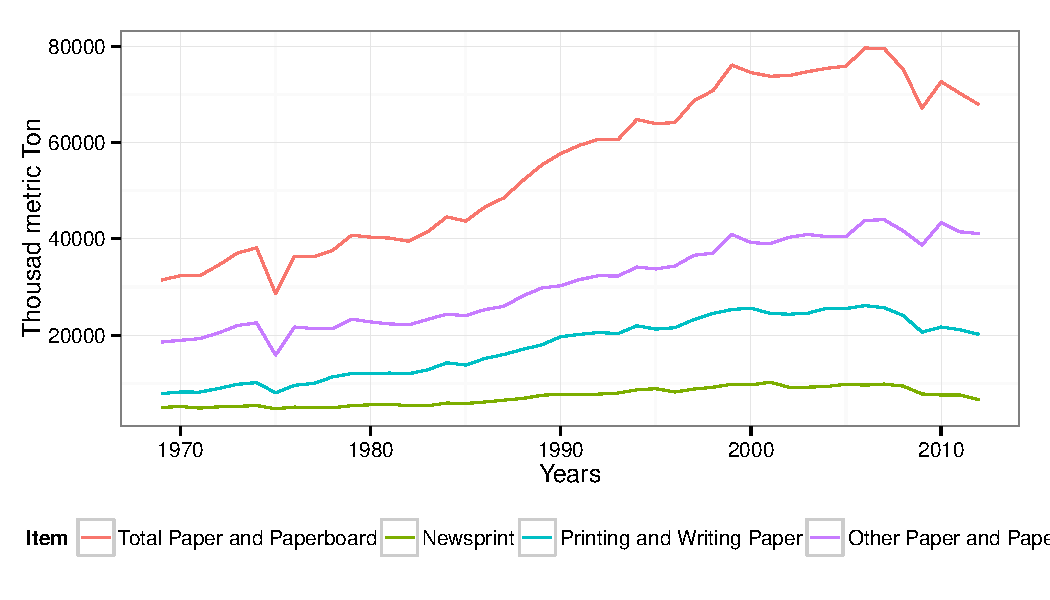
\includegraphics[width=.7\linewidth]{figure/ConsumptionEU15Extended} 

}

\caption[Consumption of paper and paperboard products in EU15, source]{Consumption of paper and paperboard products in EU15, source: FAOSTAT\label{fig:ConsumptionEU15Extended}}
\end{figure}


\end{knitrout}




\subsection{Chart of paper and paperboard prices (1969-2012)}

\begin{knitrout}
\definecolor{shadecolor}{rgb}{0.969, 0.969, 0.969}\color{fgcolor}\begin{figure}[h]


{\centering 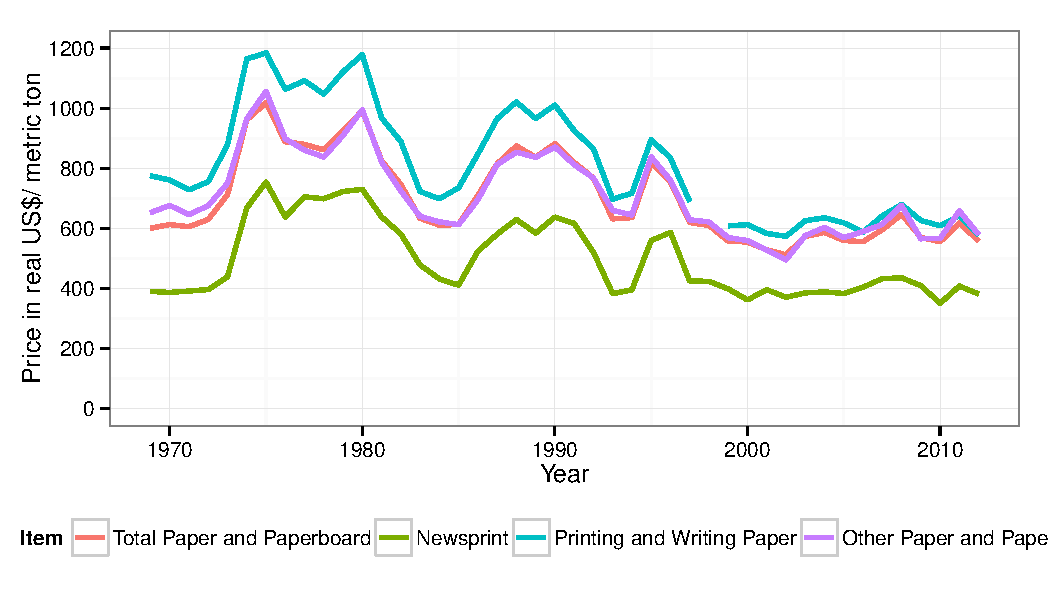
\includegraphics[width=.7\linewidth]{figure/PriceEU15Extended} 

}

\caption[Price evolution of paper and paperboard products in EU15 in USD of 1987, source]{Price evolution of paper and paperboard products in EU15 in USD of 1987, source: FAOSTAT and own calculations\label{fig:PriceEU15Extended}}
\end{figure}


\end{knitrout}



\newpage
R session info
\begin{itemize}\raggedright
  \item R version 2.15.2 (2012-10-26), \verb|i386-w64-mingw32|
  \item Base packages: base, datasets, graphics, grDevices,
    methods, stats, utils
  \item Other packages: ggplot2~0.9.3.1, knitr~1.2, plyr~1.8,
    xtable~1.7-1
  \item Loaded via a namespace (and not attached):
    colorspace~1.2-2, dichromat~2.0-0, digest~0.6.3,
    evaluate~0.4.4, formatR~0.8, grid~2.15.2, gtable~0.1.2,
    labeling~0.2, MASS~7.3-23, munsell~0.4.2, proto~0.3-10,
    RColorBrewer~1.0-5, reshape2~1.2.2, scales~0.2.3,
    stringr~0.6.2, tools~2.15.2
\end{itemize}



\end{document}
